% !Mode:: "TeX:UTF-8"
%%% Local Variables:
%%% mode: latex
%%% TeX-master: t
%%% End:

\chapter{基于关系路径的知识库补全}
\label{cha:kbc-frame}
本论文提供一种结合关系路径特征和实体属性特征的知识库补全方法。
通过提取知识库中实体的关系路径特征和实体属性特征,构建模型,进行知识库的实体关系预测。
除此之外,本论文研究了基于学习排序算法进行知识库补全的技术,在传统基于分类器模型的基础上,
提出了非线性的排序算法,对知识库候选实体对进行排序计算,获得更优的候选实体对排序集合。

图\ref{frame}展示了本部分基于逻辑符号的知识库补全算法基本框架。其中对于每个关系集合,将集合切分为训练集和测试集。
模型的训练分为两个部分:(1)特征计算,包括关系路径特征计算和实体属性特征计算两个部分;(2)模型预测,包括基于
分类模型的逻辑回归算法,基于树模型的学习排序算法,基于深度神经网络的排序算法。根据对模型评价结果,不断调整预测模型参数,
使得模型能够达到最优的结果。

\begin{figure}[H]
\begin{center}
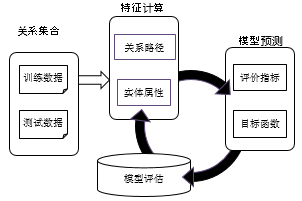
\includegraphics [width=0.5\textwidth]{frame1.PNG}
\caption{一个知识库例子}
\label{frame}
\end{center}
\end{figure}
\section{特征计算}
特征计算是知识库补全的特征抽取阶段,特征的数量和特征有效性是决定知识库补全效果的关键点之一。
给定一个完整的知识库,我们将知识库中的实体和关系分别转化为图中的顶点和边,
这样就能构建一个基于图模型的知识库补全系统。对于知识库中每种待预测的关系,
我们抽取对应关系下的实体对,将实体对的头实体和尾实体在图中进行随机游走\cite{Lao2012},
获得连接头实体和尾实体的关系路径特征,从而获得了知识库补全的关系路径特征。
给定一个目标关系r和这个关系对应的实体对集合
$$I_s=\{(s_j,t_j)|<s_j,t_j> \in KB\}$$

我们期望找出连接头尾实体对的关系路径特征。
由于连接头尾实体对之间的路径数量很大,通常需要限定关系路径的长度,
并采用随机游走算法计算选择从头实体到尾实体的关系路径,将这些路径集合作为关系路径特征。
对于能连接从头实体到尾实体的关系路径,我们记录这个关系路径的类型,作为模型预测的特征。
我们计算0-1二值化后的的路径类型,作为关系路径特征的特征值。对于每个关系抽取的关系特征,我们最终记为$V_r$ $(h_i,t_i)$作为关系路径特征,表示从头实体到尾实体有哪些关系路径进行连接。
例如对于实体对“北京师范大学,位于,北京”三元组,我们可以基于上述的关系路径抽取算法获得
“北京师范大学,位于,北京市海淀区,位于,北京”、“北京师范大学,有校长,董奇,居住在,北京”等多条路径来
获得关系“位于”对应的关系路径类型特征。

本论文通过枚举不同维度的实体属性特征,计算这些实体对在这些实体属性特征下的特征值。
属性特征抽取过程较为复杂,不仅需要考虑不同类型的属性信息不一致问题,也要研究如何处理缺失值问题。
首先对于每个实体,有着不同类型的描述特征,如一个人的信息,不仅有出生年月这种时间类型的信息,
也有年龄、性别等不同种类的属性信息。我们采用了对实体信息进行标准化的方法,
将实体对的头实体和尾实体这些不同属性特征进行归一化处理范围限定在[0,1]之间。
进行归一化后计算获得新的属性特征记为$V_l(h_i)$和$V_l (t_i)$,分别表示头实体和尾实体在所有熟悉特征下的实体属性特征向量,其中$h_i$ 和$t_i$表示给定关系l的第i个头实体和尾实体,同时我们对于头实体和尾实体进行相减计算获得$V_l(h_i-t_i )$属性值。除此之外,对于很多实体在不同特征上的缺失值,我们将缺失值进行了补0处理,期望获得更优结果。
如对于“北京师范大学”这个实体,我们抽取了他的“建校时间”、“占地面积”等所有的实体属性特征,
并计算每个实体对在这些特征下标准化后的特征值,而且将缺失属性特征补0。

\section{模型预测}
对于上述\label{sec:literal}和\label{sec:relational}抽取到的关系路径特征和实体属性特征。
传统方法构建了一个分类器模型,学习每个关系和这个关系包含的实体对集合,将预测关系问题转化成一个分类预测问题。
$E_r=\{(h_i,t_j),y_i\}^N_{i=1} $表示关系r所有的实体对集合,其中$y_i\in \{0,1\}$,其中0表示负实体对,即知识库中并不是实际存在的三元组,
1表示正实体对,表示在知识库中实际存在的实体对,通过对知识库中的实体对进行分类器模型学习,
我们可以获得测试集合中实体对的打分情况。通常这个分类器采用逻辑回归算法进行模型的训练。
具体来说,对于每个关系的实体对,传统模型采用逻辑回归学习得到的关系路径特征向量$V_r$和实体属性特征向量$V_l$。
并定义了如下的逻辑回归函数,对每个关系下的实体对集合进行评价打分。
$$f(v,w)=\frac{1}{1+e^{w(V_r \oplus  V_l)}}$$
其中w表示关系路径特征和实体属性特征的学习权重参数。经典论文采用对数似然函数进行最大似然估计,
并通过随机梯度下降算法学习这些模型的参数,除此之外,还考虑到模型的过拟合和参数正则化表示,本论文定义了如下的
学习目标函数:
$$L_r=\frac{1}{N}\sum_{i=1}^N\{(y_ilog(f(v,w_r)) + (1-y_i)log(1-f(v,w_r))\}+\alpha ||w_r||+\beta||w_r^2||$$
其中,$L_r$表示给定关系r的目标函数,$\alpha$和$\beta$ 分别是$l_1$ 和$l_2$正则化惩罚项的权重,对于每个关系我们采用随机梯度下降算法使得整个训练集对数损失最小,同时结合$l_1$ 和$l_2$防止过拟合。最终我们可以学习得到每个关系下的关系路径特征和实体属性特征的权重。


\section{评价方式}
\label{sec:metrics}
知识库补全效果的评价方法和信息检索类似,主要采用MAP和MRR\cite{Gardner2014}指标进行模型评价。同时考虑到在一个给定关系下,给定一个头实体和一系列的候选尾实体,我们希望排在前面的实体对是正确的实体对,
如果正例实体对排在负例实体对后面,则这个模型的预测效果有待改进。
所以我们借鉴了信息检索领域相关的评价方法,除了采用关键的MAP评价指标,
我们也采用了一些常见的AUC和Hit@1评价指标,希望能详尽的分析模型的有效性和可预测性。

\subsection{hit@1}
在信息检索中,hit@1表示每组三元组对应的正负实例中,正实例在该组正负例三元组中排名第一的三元组比例,
尽管这种评价指标较为简单,但可以有效衡量模型中正例三元组排在第一位比例。对于每个关系,
我们定义的的Hit@1计算公式如下:
$$hit@1=\frac{\sum_{q=1}^n{hit_q}}{n}$$
其中$hit_q$表示该关系下第$q$组实体对预测结果中,正例是否排名第一,
如果正例排名第一则$hit_q$为1,否则为0。

\subsection{平均准确率MAP}
平均准确率的英文全称是mean average precision。MAP的衡量标准比较单一,给定一个头实体和一系列候选尾实体,头尾实体对之间的关系非0即1,
我们采用局部封闭世界假设,在知识库中存在的实体对标记为1,即为正例,否则为负例。
MAP核心是利用头实体对应的相关的尾实体出现的位置来进行排序算法准确性的评估。
它反映系统在全部相关文档上性能的单值指标。系统模型计算出来的实体对越靠前(rank 越高),MAP就应该越高。否则准确率默认为0。MAP的计算公式如下:
$$MAP=\frac{\sum_{q=1}^nAP(q)}{n}$$
$$AP(q)=\frac{\sum_{i=1}^kP(i)\times rel(i)}{k}$$
其中MAP表示n个头实体和其候选尾实体的平均准确度的均值。AP(q)是一个头实体和其K个候选尾实体排序结果的评价,
如果正确的候选尾实体排在错误的候选尾实体之前,则AP值越高;
如果所有的头实体和其候选尾实体AP值越高,则模型的MAP值也就越高。
$rel(i)$在第i个实体对是预测结果时为1,否则为0。

\subsection{平均秩倒排序MRR}
MRR的全称是mean reciprocal rank。MRR通过定义第一个正确的候选尾实体来判断模型好坏,一个模型的MRR值越高,说明正确的候选尾实体在模型中排序越靠前。
MRR通常和MAP一起综合评价一个模型的好坏。
MRR的定义公式如下:
$$MRR=\frac{1}{n} \sum_{i=1}^n \frac{1}{r_i}$$

其中n表示一个关系下所有不同头实体的数目,$r_i$是每个头实体对应的正确尾实体的秩序。
MRR在很多基于问答系统的知识库补全系统\cite{West2014}中也是常见的评价方法之一。
通常情况下,基于符号逻辑的知识库补全系统中MRR值较高,多数实验结果都在0.9左右,大部分关系中的MRR实验结果差别不显著,
所以本研究的重点是关注如何显著提高知识库补全系统中关系补全的MAP指标。

\subsection{AUC}
除了常见的排序模型评价方式,我们在实验过程中也引入二分类分类器模型进行模型评价,
同时也考虑模型对正负例排序能力。AUC(Area Under Curve)被定义为ROC曲线(tpr和fpr曲线函数)下的面积,显然这个面积的数值不会大于1,同时这个值一般大于0.5。其中tpr和fpr的计算公式如下所示:
$$tpr=\frac{tp}{tp+fn}$$
$$fpr=\frac{fp}{fp+tn}$$
当你随机挑选一个正样本以及一个负样本,当前的分类算法根据计算得到的Score值将这个正样本排在负样本前面的概率就是AUC值。对所有实体对的预测得分进行排序,选择不同的阈值对正负例进行切分计算tpr和fpr的得分,从而绘制出完整的ROC曲线,并计算得到AUC的面积大小。AUC取值越大,当前的分类算法越有可能将正样本排在负样本前面,即能够更好的分类,整个模型的排序效果也更好。AUC计算公式如下所示:
$$auc=\int_{0}^{1}{tpr}*d{fpr}$$

在知识库补全预测中,无论是逻辑回归模型、支持向量机模型还是学习排序模型,
都需要关注模型的二分类的分类器性能问题。对于知识库中的实体对排序、实体对打分预测,
在评估一组实体对集合的排序秩序性能之外,也关注模型的分类性能好坏,
这些对于知识库补全算法是十分必要的。


\section{本章工作总结}
本部分介绍了本文的研究框架和总体思路。本文的基于关系路径的知识库补全算法技术,
通过抽取知识库中的实体对之间存在的关系路径类型,获得实体对基于关系路径特征的特征值,
并结合抽取的实体属性特征类型和实体属性特征值,从而获得了预测实体对之间关系的特征向量。
对于每个关系下每组实体对,我们构建机器学习预测模型,从而进行实体对之间关系的预测,
并达到补全知识库的效果。
